The third container is responsible for detecting objects for each agent. 

The detector uses OpenCV 4.3.0 built from source. To optimize performance, OpenCV has to built with \acs{cuda} backend. When building from source
additional parameters can be given with \textit{cmake}. For cuda compatibility :

\begin{verbatim}
    -DWITH_CUDA=ON \
    -DWITH_CUBLAS=ON \
    -DWITH_CUDNN=ON \
    -DOPENCV_DNN_CUDA=ON \
\end{verbatim}

All these parameters have to be set to ON for OpenCV with \acs{gpu} compatibility. When running the container the \acs{gpu} hass to be given :

\begin{verbatim}
    --gpus all
\end{verbatim}

And inside the code the prefered dnn backend has to be set. 

\begin{verbatim}
    net.setPreferableBackend(cv2.dnn.DNN_BACKEND_CUDA)
    net.setPreferableTarget(cv2.dnn.DNN_TARGET_CUDA)
\end{verbatim}

When starting the object detection, a multi process will start. 
For each \acs{uav} a detector will be made with a pre-trained tiny-yolov3 loaded into the constructor. 
The detector will then use a subsriber 
to link the camera feed from the \acs{uav} to the callback where frames from the feed will be processed with tiny-yolov3. 

When tiny-yolov3 detects an object, it will draw a rectangle around the object in a color assigned to this object. 
Next to displaying the new image with the detected objects, the detector also publishes 
the coordinates of the rectangle drawn around the found object for later usage, for example human tracking.

\begin{figure}[ht]
    \centering
    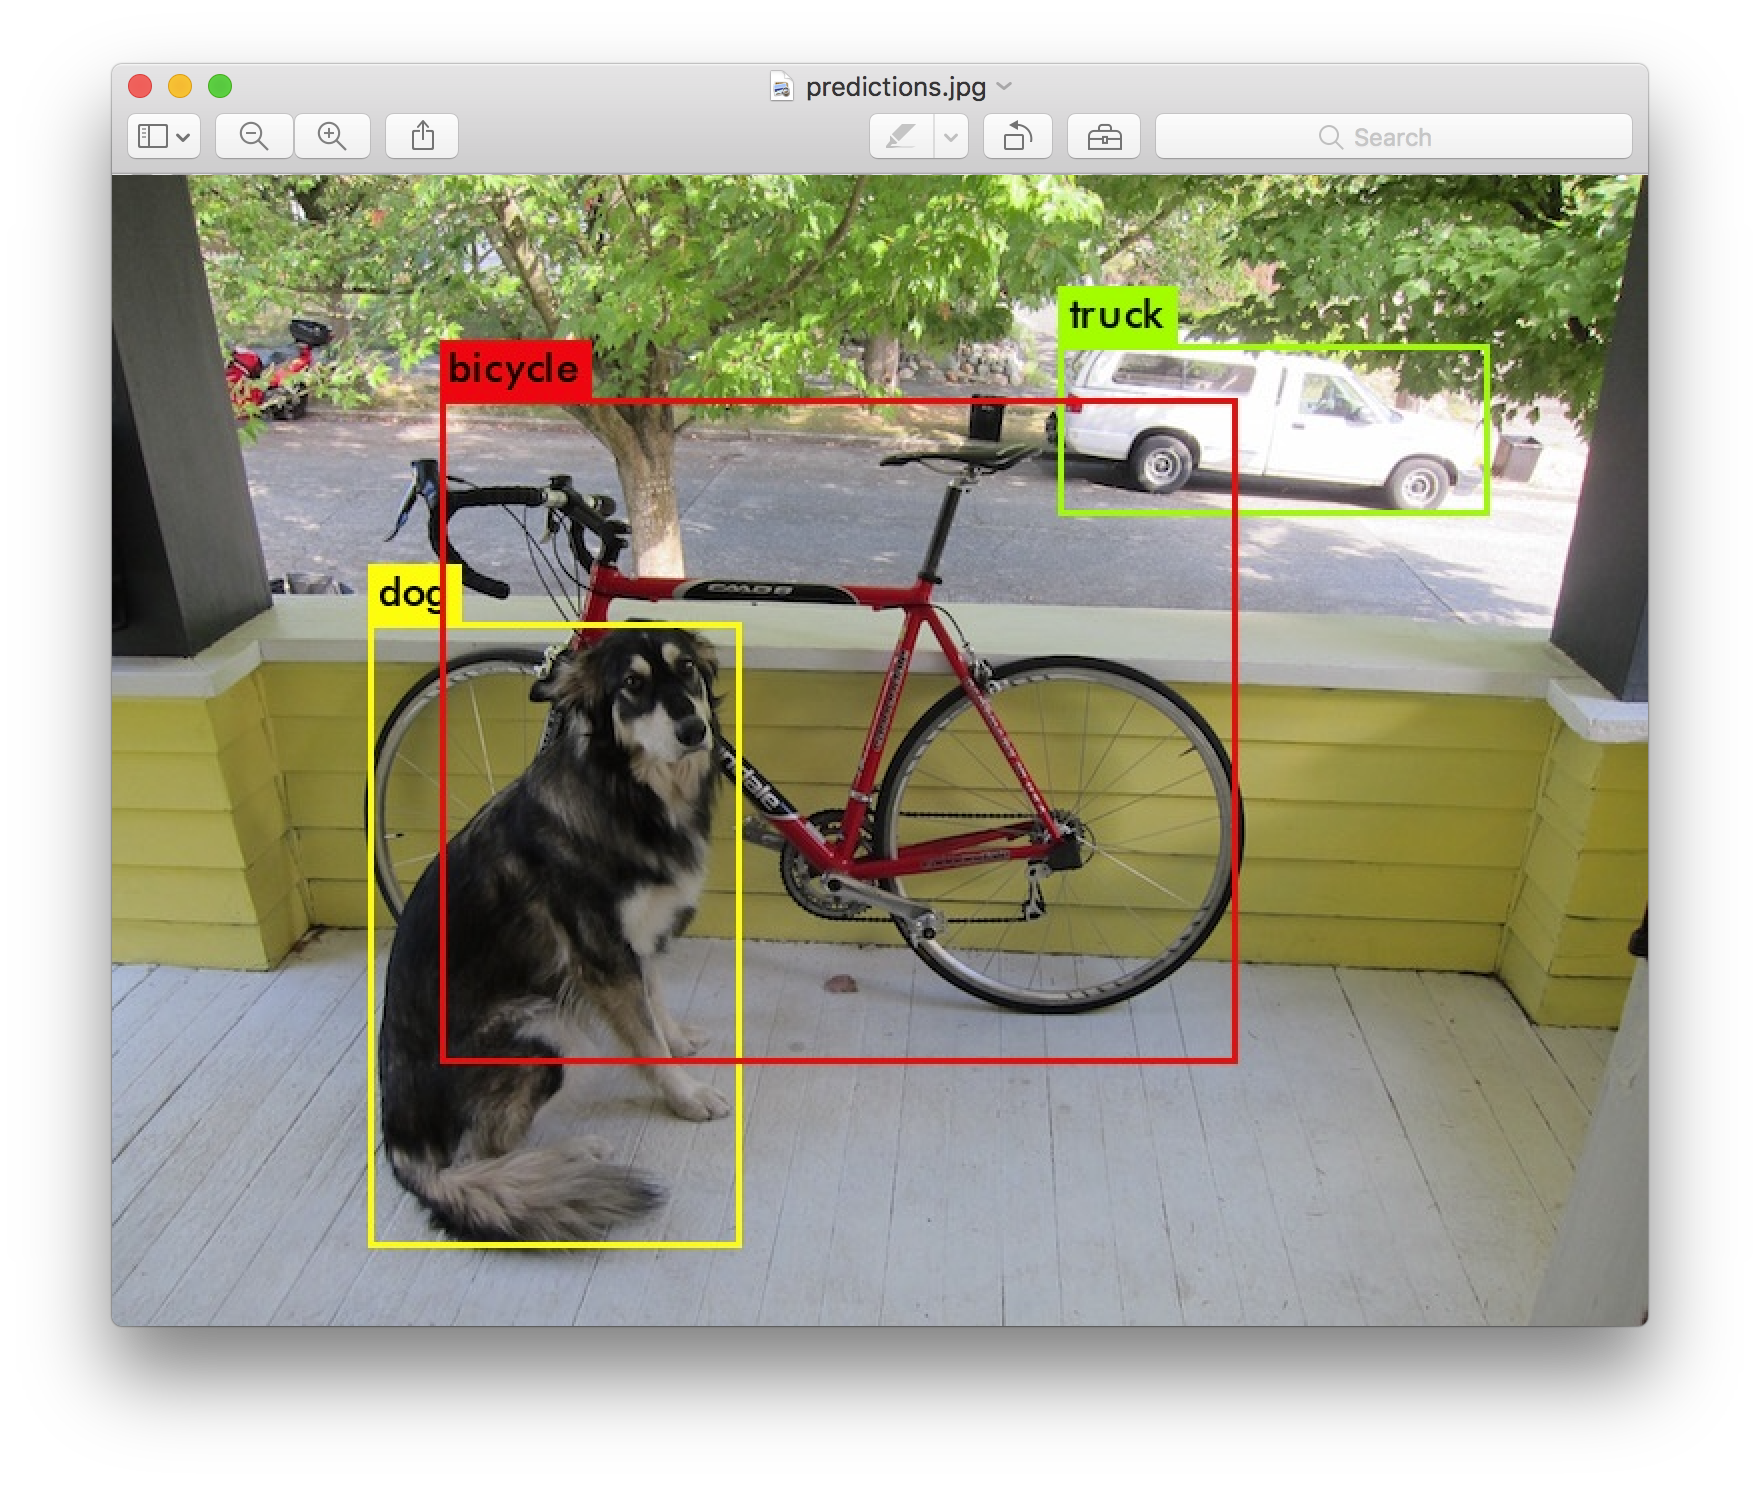
\includegraphics[scale=0.1]{darknet_obj_detection.png}
    \caption[Object detection example]{Object detection example}
\end{figure}